\documentclass[11pt,a4paper]{article}
\usepackage[utf8]{inputenc}
\usepackage[margin=1in]{geometry}
\usepackage{graphicx}
\usepackage{amsmath}
\usepackage{listings}
\usepackage{xcolor}
\usepackage{hyperref}
\usepackage{booktabs}
\usepackage{tabularx}
\usepackage{tikz}
\usepackage{float}
\usepackage{enumitem}

\usetikzlibrary{shapes.geometric, arrows, positioning, calc}

% Define colors for code listings
\definecolor{codegreen}{rgb}{0,0.6,0}
\definecolor{codegray}{rgb}{0.5,0.5,0.5}
\definecolor{codepurple}{rgb}{0.58,0,0.82}
\definecolor{backcolour}{rgb}{0.95,0.95,0.92}

% Code listing style
\lstdefinestyle{mystyle}{
    backgroundcolor=\color{backcolour},
    commentstyle=\color{codegreen},
    keywordstyle=\color{magenta},
    numberstyle=\tiny\color{codegray},
    stringstyle=\color{codepurple},
    basicstyle=\ttfamily\footnotesize,
    breakatwhitespace=false,
    breaklines=true,
    captionpos=b,
    keepspaces=true,
    numbers=left,
    numbersep=5pt,
    showspaces=false,
    showstringspaces=false,
    showtabs=false,
    tabsize=2
}
\lstset{style=mystyle}

\title{\textbf{AXI-Lite SPI Master IP Core Design Documentation} \\
\large Digital Level Application on Zynq-7000}
\author{EECE 423 Project 1}
\date{\today}

\begin{document}

\maketitle
\tableofcontents
\newpage

\section{Executive Summary}

This document provides comprehensive documentation for the design and implementation of a custom AXI-Lite SPI Master IP core integrated with the Xilinx Zynq-7000 SoC. The project implements a digital level (tilt sensor) using the Digilent PmodACL (ADXL345 accelerometer) interfaced via SPI communication.

\subsection{Key Components}
\begin{itemize}[leftmargin=*]
    \item \textbf{Hardware Platform:} Xilinx ZedBoard (xc7z020clg484-1)
    \item \textbf{Custom IP Core:} AXI-Lite SPI Master supporting modes 0-3
    \item \textbf{Sensor:} ADXL345 3-axis accelerometer (SPI interface)
    \item \textbf{Software:} Interrupt-driven embedded C application
    \item \textbf{Update Rate:} 500ms timer-driven data acquisition
\end{itemize}

\section{System Architecture}

\subsection{Hardware Block Diagram}

The system architecture consists of three main components interconnected via the AMBA AXI protocol:

\begin{figure}[H]
\centering
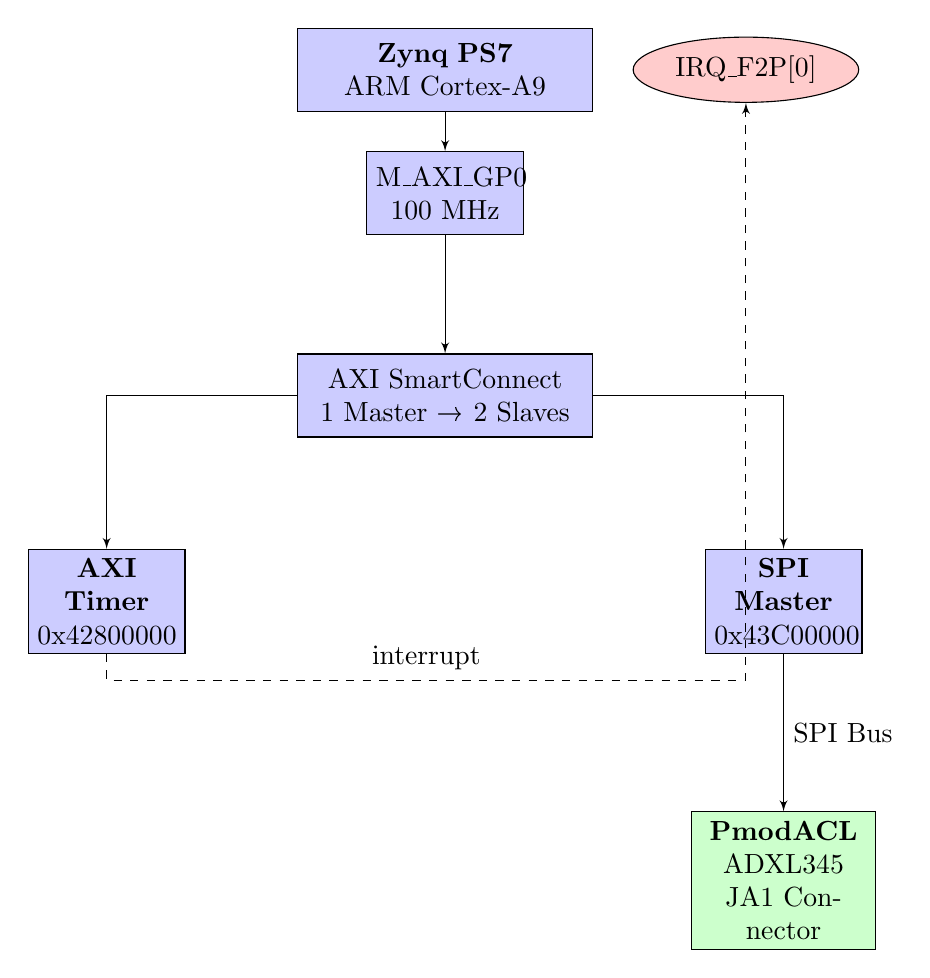
\begin{tikzpicture}[
    block/.style={rectangle, draw, fill=blue!20, text width=5em, text centered, minimum height=3em},
    wideblock/.style={rectangle, draw, fill=blue!20, text width=10em, text centered, minimum height=3em},
    sensor/.style={rectangle, draw, fill=green!20, text width=6em, text centered, minimum height=3em},
    line/.style={draw, -latex'},
    cloud/.style={draw, ellipse, fill=red!20, minimum height=2em}
]

% Zynq PS
\node [wideblock] (ps) {\textbf{Zynq PS7} \\ ARM Cortex-A9};
\node [block, below=0.5cm of ps] (axi) {M\_AXI\_GP0 \\ 100 MHz};
\node [cloud, right=0.5cm of ps] (irq) {IRQ\_F2P[0]};

% AXI Interconnect
\node [wideblock, below=1.5cm of axi] (interconnect) {AXI SmartConnect \\ 1 Master → 2 Slaves};

% Timer
\node [block, below left=2cm of interconnect] (timer) {\textbf{AXI Timer} \\ 0x42800000};

% SPI Master
\node [block, below right=2cm of interconnect] (spi) {\textbf{SPI Master} \\ 0x43C00000};

% Sensor
\node [sensor, below=2cm of spi] (accel) {\textbf{PmodACL} \\ ADXL345 \\ JA1 Connector};

% Connections
\draw [line] (ps) -- (axi);
\draw [line] (axi) -- (interconnect);
\draw [line] (interconnect) -| (timer);
\draw [line] (interconnect) -| (spi);
\draw [line, dashed] (timer) -- ++(0,-1) -| node[near start, above] {interrupt} (irq);
\draw [line] (spi) -- node[right] {SPI Bus} (accel);

\end{tikzpicture}
\caption{System Block Diagram}
\label{fig:block_diagram}
\end{figure}

\subsection{Physical Pin Mapping}

The SPI interface connects to the ZedBoard's JA1 Pmod connector with the following pin assignments:

\begin{table}[H]
\centering
\caption{SPI Pin Mapping to ZedBoard JA1 Connector}
\label{tab:pin_mapping}
\begin{tabular}{@{}lllll@{}}
\toprule
\textbf{Signal} & \textbf{IP Port} & \textbf{FPGA Pin} & \textbf{Pmod Pin} & \textbf{Description} \\ \midrule
CS & o\_SPI\_CS\_n & Y11 & 1 & Chip Select (active low) \\
MOSI & o\_SPI\_MOSI & AA11 & 2 & Master Out Slave In \\
MISO & i\_SPI\_MISO & Y10 & 3 & Master In Slave Out \\
SCK & o\_SPI\_Clk & AA9 & 4 & Serial Clock (4 MHz) \\
GND & --- & GND & 5 & Ground \\
VCC & --- & 3.3V & 6 & Power Supply (3.3V) \\ \bottomrule
\end{tabular}
\end{table}

\textbf{Critical Note:} The PmodACL must be connected with the IC facing \textbf{UP} for correct pin alignment.

\section{Register Map}

\subsection{SPI Master IP Register Map}

The SPI Master IP core implements an AXI-Lite slave interface with five memory-mapped registers at base address \texttt{0x43C00000}.

\begin{table}[H]
\centering
\caption{SPI Master IP Register Map}
\label{tab:register_map}
\small
\begin{tabularx}{\textwidth}{@{}llX@{}}
\toprule
\textbf{Offset} & \textbf{Register Name} & \textbf{Description} \\ \midrule

\texttt{0x00} & CONTROL\_REG & \textbf{SPI Mode and Clock Configuration} \\
& & [1:0] SPI Mode: 0=Mode0, 1=Mode1, 2=Mode2, 3=Mode3 \\
& & [31:16] Clock Scale: Divider value (100MHz / scale) \\
& & \textit{Default:} \texttt{0x00190003} (Mode 3, Scale 25 → 4MHz) \\
\addlinespace

\texttt{0x04} & CONFIG\_REG & \textbf{Transaction Configuration} \\
& & [2:0] CS Inactive Clocks: Delay between transactions \\
& & [12:8] TX Count: Bytes per transaction (1-16) \\
& & \textit{Default:} \texttt{0x00000101} (CS\_Inactive=1, TX\_Count=1) \\
\addlinespace

\texttt{0x08} & TX\_DATA\_REG & \textbf{Transmit Data Register (Write-Only)} \\
& & [7:0] TX Byte: Data to transmit \\
& & \textit{Note:} Writing to this register triggers transmission \\
\addlinespace

\texttt{0x0C} & RX\_DATA\_REG & \textbf{Receive Data Register (Read-Only)} \\
& & [7:0] RX Byte: Last received byte from SPI \\
\addlinespace

\texttt{0x10} & STATUS\_REG & \textbf{Status Register (Read-Only)} \\
& & [0] TX Ready: 1=ready for new data, 0=busy \\
& & [1] RX Valid: 1=new data available \\
& & [11:8] RX Count: Current byte index (0-15) \\

\bottomrule
\end{tabularx}
\end{table}

\subsection{Register Usage Examples}

\subsubsection{Initialization Sequence}
\begin{lstlisting}[language=C, caption=SPI Master Initialization]
// Configure for SPI Mode 3, 4 MHz clock
Xil_Out32(SPI_BASE + 0x00, 0x00190003);  // CONTROL_REG
// Configure for 1-byte transactions, 1 clock CS inactive
Xil_Out32(SPI_BASE + 0x04, 0x00000101);  // CONFIG_REG
\end{lstlisting}

\subsubsection{Data Transmission}
\begin{lstlisting}[language=C, caption=SPI Transaction Example]
// Wait for TX_READY
while (!(Xil_In32(SPI_BASE + 0x10) & 0x01));
// Send data byte
Xil_Out32(SPI_BASE + 0x08, 0x2D);  // TX_DATA_REG
// Wait for RX_VALID
while (!(Xil_In32(SPI_BASE + 0x10) & 0x02));
// Read received byte
u8 data = Xil_In32(SPI_BASE + 0x0C) & 0xFF;  // RX_DATA_REG
\end{lstlisting}

\subsection{ADXL345 Accelerometer Register Map}

The ADXL345 contains registers for configuration and data readout accessed via SPI:

\begin{table}[H]
\centering
\caption{ADXL345 Key Registers}
\label{tab:adxl345_registers}
\begin{tabular}{@{}llp{8cm}@{}}
\toprule
\textbf{Address} & \textbf{Register} & \textbf{Description} \\ \midrule
\texttt{0x00} & DEVID & Device ID (always reads \texttt{0xE5}) \\
\texttt{0x2D} & POWER\_CTL & Power control register. Bit 3: Measure mode enable \\
\texttt{0x31} & DATA\_FORMAT & Data format control. Set to \texttt{0x09}: ±4g range, full resolution \\
\texttt{0x32} & DATAX0 & X-axis data LSB \\
\texttt{0x33} & DATAX1 & X-axis data MSB \\
\texttt{0x34} & DATAY0 & Y-axis data LSB \\
\texttt{0x35} & DATAY1 & Y-axis data MSB \\
\texttt{0x36} & DATAZ0 & Z-axis data LSB \\
\texttt{0x37} & DATAZ1 & Z-axis data MSB \\ \bottomrule
\end{tabular}
\end{table}

\subsubsection{ADXL345 SPI Protocol}

The ADXL345 uses a specific command format where the command byte encodes the operation:

\begin{itemize}
    \item \textbf{Bit [7]:} Read/Write (1=Read, 0=Write)
    \item \textbf{Bit [6]:} Multi-byte (1=Multi-byte, 0=Single-byte)
    \item \textbf{Bits [5:0]:} Register address
\end{itemize}

\textbf{Examples:}
\begin{itemize}
    \item Write to POWER\_CTL (0x2D): Command = \texttt{0x2D}
    \item Read from DEVID (0x00): Command = \texttt{0x80}
    \item Multi-byte read from DATAX0 (0x32): Command = \texttt{0xF2}
\end{itemize}

\section{HDL Architecture and Design Decisions}

\subsection{Module Hierarchy}

The SPI Master IP consists of three Verilog modules organized hierarchically:

\begin{figure}[H]
\centering
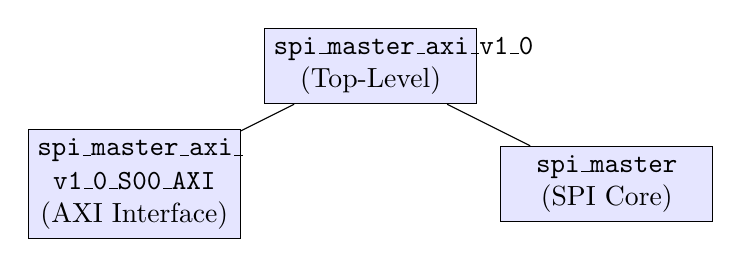
\begin{tikzpicture}[
    level 1/.style={sibling distance=6cm},
    level 2/.style={sibling distance=3cm},
    box/.style={rectangle, draw, fill=blue!10, text width=7em, text centered, minimum height=2.5em}
]
\node [box] {\texttt{spi\_master\_axi\_v1\_0} \\ (Top-Level)}
    child {node [box] {\texttt{spi\_master\_axi\_ \\ v1\_0\_S00\_AXI} \\ (AXI Interface)}}
    child {node [box] {\texttt{spi\_master} \\ (SPI Core)}};
\end{tikzpicture}
\caption{HDL Module Hierarchy}
\end{figure}

\subsection{SPI Core State Machine}

The \texttt{spi\_master.v} module implements the core SPI logic using a finite state machine:

\begin{table}[H]
\centering
\caption{SPI Master State Machine}
\label{tab:state_machine}
\begin{tabular}{@{}lp{10cm}@{}}
\toprule
\textbf{State} & \textbf{Description} \\ \midrule
IDLE & Waiting for \texttt{TX\_DV} signal to initiate transfer \\
WAIT\_HALF & (Mode 1/3 only) Wait half clock period before first data output \\
TRANSFER & Active SPI transfer with clock generation and data shifting \\
CS\_INACTIVE & CS de-assertion delay between consecutive transactions \\ \bottomrule
\end{tabular}
\end{table}

\begin{lstlisting}[language=Verilog, caption=SPI State Machine Declaration]
localparam IDLE = 3'd0;
localparam WAIT_HALF = 3'd1;
localparam TRANSFER = 3'd2;
localparam CS_INACTIVE = 3'd3;

reg [2:0] r_sm_cs;  // Current state
\end{lstlisting}

\subsection{Clock Generation Logic}

\textbf{Design Decision:} Parameterized clock divider for flexible SPI clock rates.

\begin{itemize}
    \item \textbf{Input Clock:} 100 MHz (from Zynq PS)
    \item \textbf{SPI Clock:} Configurable via \texttt{i\_clk\_scale} register
    \item \textbf{Selected Configuration:} Scale factor = 25 → 4 MHz SPI clock
    \item \textbf{Rationale:} ADXL345 supports up to 5 MHz; 4 MHz provides margin
\end{itemize}

The clock generator creates \texttt{leading\_edge} and \texttt{trailing\_edge} strobes based on the configured SPI mode:

\begin{lstlisting}[language=Verilog, caption=SPI Mode Configuration]
wire CPOL = i_spi_mode[1];  // Clock polarity
wire CPHA = i_spi_mode[0];  // Clock phase

wire sample_edge = (CPHA == 0) ? leading_edge : trailing_edge;
wire shift_edge = (CPHA == 0) ? trailing_edge : leading_edge;
\end{lstlisting}

\subsection{Multi-Byte Transaction Support}

\textbf{Design Decision:} Support 1-16 byte transactions for efficient multi-register reads.

The SPI core includes byte counting logic to handle multi-byte transactions required for reading all three accelerometer axes (6 bytes total):

\begin{lstlisting}[language=Verilog, caption=Byte Counter Logic]
input wire [4:0] i_tx_count;        // Number of bytes to transfer
output reg [3:0] o_rx_count;        // Current byte index (0-15)
output reg o_tx_ready;              // Ready for next byte
\end{lstlisting}

This eliminates the overhead of re-asserting CS between each byte, improving throughput.

\subsection{AXI-Lite Interface Design}

\textbf{Design Decision:} AXI-Lite (not AXI4-Full) for simplicity and lower resource usage.

The AXI interface module (\texttt{spi\_master\_axi\_v1\_0\_S00\_AXI.v}) implements:

\begin{itemize}
    \item Standard AXI4-Lite slave protocol
    \item 5 × 32-bit memory-mapped registers
    \item Automatic TX\_DV pulse generation on write to TX\_DATA\_REG
    \item Status register auto-update from SPI core signals
    \item Default register values on reset
\end{itemize}

\begin{lstlisting}[language=Verilog, caption=TX\_DV Pulse Generation]
always @(posedge S_AXI_ACLK) begin
    if (!S_AXI_ARESETN) begin
        tx_dv <= 1'b0;
    end else begin
        // Generate single-cycle pulse on TX_DATA_REG write
        if (axi_awaddr == 3'h2 && axi_wready && S_AXI_WVALID) begin
            tx_dv <= 1'b1;
        end else begin
            tx_dv <= 1'b0;
        end
    end
end
\end{lstlisting}

\section{Software Architecture}

\subsection{Software Stack}

The embedded software is organized in a layered architecture:

\begin{figure}[H]
\centering
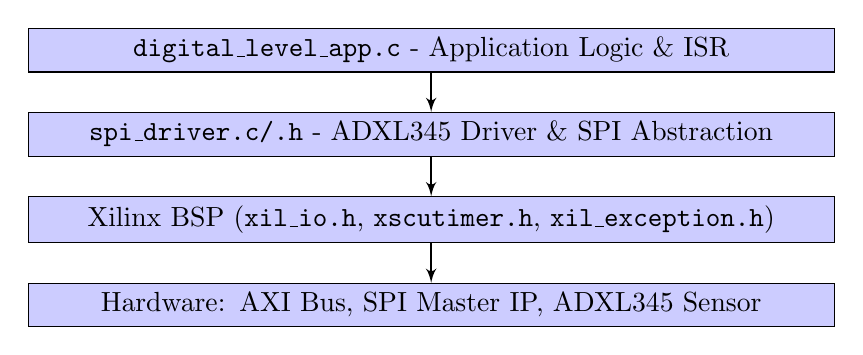
\begin{tikzpicture}[
    box/.style={rectangle, draw, fill=blue!20, text width=10cm, text centered, minimum height=1.5em},
    node distance=0.5cm
]
\node [box] (app) {\texttt{digital\_level\_app.c} - Application Logic \& ISR};
\node [box, below=of app] (driver) {\texttt{spi\_driver.c/.h} - ADXL345 Driver \& SPI Abstraction};
\node [box, below=of driver] (bsp) {Xilinx BSP (\texttt{xil\_io.h}, \texttt{xscutimer.h}, \texttt{xil\_exception.h})};
\node [box, below=of bsp] (hw) {Hardware: AXI Bus, SPI Master IP, ADXL345 Sensor};

\draw [-latex', thick] (app) -- (driver);
\draw [-latex', thick] (driver) -- (bsp);
\draw [-latex', thick] (bsp) -- (hw);
\end{tikzpicture}
\caption{Software Layered Architecture}
\end{figure}

\subsection{Driver Layer Design Decisions}

\subsubsection{Timeout Protection}

\textbf{Problem:} Infinite loops in polling can hang the system if hardware is non-responsive.

\textbf{Solution:} All polling functions include timeout counters with diagnostic output:

\begin{lstlisting}[language=C, caption=Timeout-Protected Wait Function]
void SPI_WaitReady(u32 BaseAddress)
{
    u32 timeout = 100000;
    while (!SPI_IsReady(BaseAddress) && timeout > 0) {
        timeout--;
    }
    if (timeout == 0) {
        u32 status = Xil_In32(BaseAddress + SPI_STATUS_REG_OFFSET);
        xil_printf("WARNING: SPI_WaitReady timeout! Status=0x%08X\r\n", status);
    }
}
\end{lstlisting}

\textbf{Rationale:} Essential during development to detect hardware configuration errors early.

\subsubsection{ADXL345 Protocol Abstraction}

The driver provides high-level functions hiding the SPI command byte construction:

\begin{lstlisting}[language=C, caption=ADXL345 Read Function]
u8 ADXL345_ReadRegister(u32 BaseAddress, u8 reg_addr)
{
    SPI_WaitReady(BaseAddress);

    // Send read command (bit 7 = 1)
    u8 command = 0x80 | (reg_addr & 0x3F);
    Xil_Out32(BaseAddress + SPI_TX_DATA_REG_OFFSET, command);

    SPI_WaitValid(BaseAddress);
    Xil_In32(BaseAddress + SPI_RX_DATA_REG_OFFSET);  // Dummy read

    // Send dummy byte to clock in data
    Xil_Out32(BaseAddress + SPI_TX_DATA_REG_OFFSET, 0x00);

    SPI_WaitValid(BaseAddress);
    return Xil_In32(BaseAddress + SPI_RX_DATA_REG_OFFSET) & 0xFF;
}
\end{lstlisting}

\subsection{Application Layer Design Decisions}

\subsubsection{Interrupt-Driven Data Acquisition}

\textbf{Design Decision:} Use timer interrupts rather than continuous polling.

\textbf{Benefits:}
\begin{itemize}
    \item Reduces CPU overhead (ARM cores can enter low-power states)
    \item Provides deterministic 500ms update rate
    \item Simplifies main loop logic
\end{itemize}

\begin{lstlisting}[language=C, caption=Timer Interrupt Service Routine]
void TimerInterruptHandler(void *CallBackRef, u8 TmrCtrNumber)
{
    s16 x, y, z;

    // Read all three axes from ADXL345
    ADXL345_ReadAccel(SPI_MASTER_BASEADDR, &x, &y, &z);

    // Update global variables (shared with main loop)
    g_accel_x = x;
    g_accel_y = y;
    g_accel_z = z;
    g_angle = ADXL345_CalculateAngle(y, z);
    g_new_data = 1;  // Signal main loop
}
\end{lstlisting}

\textbf{Timer Configuration:} 50,000,000 clock cycles at 100 MHz = 500ms period

\subsubsection{Angle Calculation Algorithm}

The application calculates the inclination angle in the Y-Z plane using the arctangent:

\begin{equation}
\theta = \arctan\left(\frac{Y}{\sqrt{Y^2 + Z^2}}\right) \times \frac{180}{\pi}
\end{equation}

\begin{lstlisting}[language=C, caption=Angle Calculation]
float ADXL345_CalculateAngle(s16 y, s16 z)
{
    float y_f = (float)y;
    float z_f = (float)z;

    // Calculate angle in radians
    float angle_rad = atan2(y_f, sqrt(y_f*y_f + z_f*z_f));

    // Convert to degrees
    return angle_rad * (180.0 / 3.14159);
}
\end{lstlisting}

\section{Implementation Steps}

\subsection{Phase 1: HDL Development and IP Packaging}

\subsubsection{Step 1.1: Write Verilog Modules}

Three Verilog files were created:
\begin{enumerate}
    \item \texttt{spi\_master.v} (241 lines) - Core SPI logic with state machine
    \item \texttt{spi\_master\_axi\_v1\_0\_S00\_AXI.v} (422 lines) - AXI-Lite interface
    \item \texttt{spi\_master\_axi\_v1\_0.v} (135 lines) - Top-level wrapper
\end{enumerate}

\subsubsection{Step 1.2: Package as Vivado IP}

Using the TCL script \texttt{package\_ip.tcl}, the modules are packaged as a reusable IP core:

\begin{lstlisting}[language=bash, caption=IP Packaging Command]
vivado -mode batch -source package_ip.tcl
\end{lstlisting}

\textbf{Key IP Properties:}
\begin{itemize}
    \item Vendor: \texttt{user.org}
    \item Library: \texttt{user}
    \item Name: \texttt{spi\_master\_axi}
    \item Version: 1.0
    \item Display Name: \texttt{SPI Master AXI v1.0}
\end{itemize}

\subsection{Phase 2: Vivado Block Design}

\subsubsection{Step 2.1: Create Project}

Execute the comprehensive project creation script:

\begin{lstlisting}[language=bash, caption=Project Creation]
vivado -mode batch -source create_vivado_project.tcl
\end{lstlisting}

\subsubsection{Step 2.2: Configure Zynq PS7}

The Zynq Processing System IP is configured with:

\begin{itemize}
    \item \textbf{Clock:} FCLK\_CLK0 enabled at 100 MHz
    \item \textbf{AXI Interface:} M\_AXI\_GP0 enabled (32-bit, 100 MHz)
    \item \textbf{Interrupts:} IRQ\_F2P[0:0] enabled for timer
    \item \textbf{DDR:} Default configuration (512 MB)
    \item \textbf{UART:} UART1 enabled for terminal output
\end{itemize}

\subsubsection{Step 2.3: Add and Connect IP Cores}

The following IP cores are instantiated and connected:

\begin{enumerate}
    \item \textbf{AXI SmartConnect} (1 master → 2 slaves)
    \item \textbf{AXI Timer} (configured for 500ms interrupts)
    \item \textbf{SPI Master AXI} (custom IP)
    \item \textbf{Processor System Reset} (reset synchronization)
\end{enumerate}

\subsubsection{Step 2.4: Memory Address Assignment}

\begin{table}[H]
\centering
\caption{AXI Peripheral Address Map}
\begin{tabular}{@{}lll@{}}
\toprule
\textbf{Peripheral} & \textbf{Base Address} & \textbf{Range} \\ \midrule
SPI Master IP & \texttt{0x43C00000} & 64K \\
AXI Timer & \texttt{0x42800000} & 64K \\ \bottomrule
\end{tabular}
\end{table}

\subsubsection{Step 2.5: Critical Fix - Make SPI Ports External}

\textbf{CRITICAL DESIGN STEP:} The SPI signals must be exposed as external ports in the block design.

This is accomplished using the \texttt{fix\_block\_design.tcl} script:

\begin{lstlisting}[language=tcl, caption=Making Ports External]
# Make SPI ports external
make_bd_pins_external [get_bd_pins spi_master_axi_0/o_SPI_Clk]
make_bd_pins_external [get_bd_pins spi_master_axi_0/o_SPI_MOSI]
make_bd_pins_external [get_bd_pins spi_master_axi_0/i_SPI_MISO]
make_bd_pins_external [get_bd_pins spi_master_axi_0/o_SPI_CS_n]

# Rename to clean names
set_property name o_SPI_Clk [get_bd_ports o_SPI_Clk_0]
set_property name o_SPI_MOSI [get_bd_ports o_SPI_MOSI_0]
set_property name i_SPI_MISO [get_bd_ports i_SPI_MISO_0]
set_property name o_SPI_CS_n [get_bd_ports o_SPI_CS_n_0]
\end{lstlisting}

\textbf{Failure Mode:} If this step is skipped, Vivado will issue warnings like:
\begin{verbatim}
[BD 41-759] No ports matched 'o_SPI_Clk'
\end{verbatim}
and the constraint file will fail to apply, leaving the signals unconnected.

\subsubsection{Step 2.6: Apply Pin Constraints}

The file \texttt{constraints/zedboard\_pmod\_ja1.xdc} assigns FPGA pins:

\begin{lstlisting}[caption=Pin Constraint File Excerpt]
# SPI Clock
set_property PACKAGE_PIN AA9 [get_ports o_SPI_Clk]
set_property IOSTANDARD LVCMOS33 [get_ports o_SPI_Clk]

# SPI MOSI
set_property PACKAGE_PIN AA11 [get_ports o_SPI_MOSI]
set_property IOSTANDARD LVCMOS33 [get_ports o_SPI_MOSI]

# SPI MISO
set_property PACKAGE_PIN Y10 [get_ports i_SPI_MISO]
set_property IOSTANDARD LVCMOS33 [get_ports i_SPI_MISO]

# SPI CS
set_property PACKAGE_PIN Y11 [get_ports o_SPI_CS_n]
set_property IOSTANDARD LVCMOS33 [get_ports o_SPI_CS_n]
\end{lstlisting}

\subsubsection{Step 2.7: Generate Bitstream}

The complete build process:
\begin{enumerate}
    \item Validate block design
    \item Create HDL wrapper (auto-generated top-level)
    \item Run Synthesis
    \item Run Implementation (Place \& Route)
    \item Generate Bitstream (.bit file)
\end{enumerate}

\subsection{Phase 3: Software Development}

\subsubsection{Step 3.1: Export Hardware}

Export the hardware platform to Vitis:
\begin{itemize}
    \item File → Export → Export Hardware
    \item Include bitstream: \textbf{Yes}
    \item Output: \texttt{design\_1\_wrapper.xsa}
\end{itemize}

\subsubsection{Step 3.2: Create Vitis Workspace}

\begin{enumerate}
    \item Launch Vitis IDE
    \item Create platform project from XSA file
    \item Build platform (generates \texttt{xparameters.h})
\end{enumerate}

\subsubsection{Step 3.3: Verify xparameters.h}

The auto-generated header must contain correct base addresses:

\begin{lstlisting}[language=C, caption=Expected xparameters.h Content]
#define XPAR_SPI_MASTER_AXI_0_S00_AXI_BASEADDR 0x43C00000
#define XPAR_AXI_TIMER_0_BASEADDR 0x42800000
\end{lstlisting}

\textbf{Compatibility Issue:} Newer Vitis versions may omit \texttt{DEVICE\_ID} macros. The application includes fallback definitions:

\begin{lstlisting}[language=C, caption=Compatibility Layer]
#ifndef XPAR_SCUTIMER_DEVICE_ID
    #warning "XPAR_SCUTIMER_DEVICE_ID not defined, using default 0"
    #define XPAR_SCUTIMER_DEVICE_ID 0
#endif
\end{lstlisting}

\subsubsection{Step 3.4: Implement Driver Layer}

Files: \texttt{spi\_driver.c} and \texttt{spi\_driver.h}

Key functions implemented:
\begin{itemize}
    \item \texttt{SPI\_Init()} - Configure SPI mode and clock
    \item \texttt{SPI\_WaitReady()} - Poll TX\_READY with timeout
    \item \texttt{SPI\_WaitValid()} - Poll RX\_VALID with timeout
    \item \texttt{ADXL345\_Init()} - Configure accelerometer
    \item \texttt{ADXL345\_ReadRegister()} - Single-byte SPI read
    \item \texttt{ADXL345\_WriteRegister()} - Single-byte SPI write
    \item \texttt{ADXL345\_ReadAccel()} - Read X, Y, Z axes (6 bytes)
\end{itemize}

\subsubsection{Step 3.5: Implement Application}

File: \texttt{digital\_level\_app.c}

Application flow:
\begin{enumerate}
    \item Initialize peripherals (SPI, Timer, Interrupts)
    \item Configure ADXL345 (power on, set range)
    \item Verify device ID (should read 0xE5)
    \item Start timer (generates interrupt every 500ms)
    \item Main loop: Check for new data, display angle
\end{enumerate}

\subsection{Phase 4: Integration and Testing}

\subsubsection{Step 4.1: Program FPGA}

\begin{enumerate}
    \item Connect ZedBoard via USB (JTAG and UART)
    \item Open hardware manager in Vivado
    \item Program device with bitstream
    \item Verify "Programming successful" message
\end{enumerate}

\subsubsection{Step 4.2: Build and Run Application}

\begin{enumerate}
    \item Build application in Vitis (Release configuration)
    \item Launch on hardware (Single Application Debug)
    \item Open serial terminal (115200 baud, 8N1)
\end{enumerate}

\subsubsection{Step 4.3: Verification Checklist}

\begin{table}[H]
\centering
\caption{System Verification Steps}
\begin{tabular}{@{}lp{8cm}@{}}
\toprule
\textbf{Test} & \textbf{Expected Result} \\ \midrule
Device ID & Read 0xE5 from register 0x00 \\
STATUS Register & Bit 0 (TX\_READY) = 1 after reset \\
SPI Clock & 4 MHz measured on oscilloscope \\
Accelerometer Data & Non-zero values when board tilted \\
Angle Display & Updates every 500ms, changes with tilt \\
Timeout Messages & None (indicates healthy hardware) \\ \bottomrule
\end{tabular}
\end{table}

\section{Key Design Decisions Summary}

\subsection{Hardware Design Decisions}

\begin{enumerate}
    \item \textbf{AXI-Lite vs. AXI4-Full}
    \begin{itemize}
        \item \textit{Decision:} Use AXI-Lite
        \item \textit{Rationale:} Simple register interface; no burst transfers needed
        \item \textit{Benefit:} Lower resource utilization, simpler verification
    \end{itemize}

    \item \textbf{Single Clock Domain}
    \begin{itemize}
        \item \textit{Decision:} Entire design operates at 100 MHz
        \item \textit{Rationale:} Eliminates clock domain crossing (CDC) complexity
        \item \textit{Trade-off:} SPI clock generated by counter, not separate PLL
    \end{itemize}

    \item \textbf{SPI Mode 3 (CPOL=1, CPHA=1)}
    \begin{itemize}
        \item \textit{Requirement:} ADXL345 datasheet specifies Mode 3
        \item \textit{Implementation:} Configurable via CONTROL\_REG for flexibility
    \end{itemize}

    \item \textbf{4 MHz SPI Clock}
    \begin{itemize}
        \item \textit{Decision:} Use 4 MHz (clock scale = 25)
        \item \textit{Rationale:} ADXL345 supports up to 5 MHz; 4 MHz provides margin
        \item \textit{Alternative:} Could use 5 MHz (scale = 20) for faster throughput
    \end{itemize}

    \item \textbf{External Port Exposure}
    \begin{itemize}
        \item \textit{Critical:} SPI ports must be made external in block design
        \item \textit{Common Error:} Forgetting this step causes constraint failures
        \item \textit{Solution:} Automated via TCL script
    \end{itemize}
\end{enumerate}

\subsection{Software Design Decisions}

\begin{enumerate}
    \item \textbf{Polling with Timeout vs. Infinite Polling}
    \begin{itemize}
        \item \textit{Decision:} All polling includes 100,000-iteration timeout
        \item \textit{Rationale:} Prevents system hang during hardware debug
        \item \textit{Trade-off:} Slight overhead, but essential for diagnostics
    \end{itemize}

    \item \textbf{Interrupt-Driven vs. Continuous Polling}
    \begin{itemize}
        \item \textit{Decision:} Use timer interrupts for data acquisition
        \item \textit{Benefits:} Lower CPU usage, deterministic timing
        \item \textit{Alternative:} Could poll accelerometer data-ready interrupt
    \end{itemize}

    \item \textbf{Verbose Debug Output}
    \begin{itemize}
        \item \textit{Decision:} Extensive \texttt{xil\_printf()} statements
        \item \textit{Rationale:} Essential during development for troubleshooting
        \item \textit{Production:} Could be removed or made conditional
    \end{itemize}

    \item \textbf{Little-Endian Data Handling}
    \begin{itemize}
        \item \textit{Fact:} ADXL345 transmits LSB first (little-endian)
        \item \textit{Implementation:} Manual byte assembly in driver
        \item \textit{Code:} \texttt{value = (MSB << 8) | LSB}
    \end{itemize}
\end{enumerate}

\section{Common Issues and Troubleshooting}

\subsection{Issue 1: Missing SPI Ports}

\textbf{Symptom:} Vivado constraint warnings:
\begin{verbatim}
[BD 41-759] No ports matched 'o_SPI_Clk'
\end{verbatim}

\textbf{Root Cause:} SPI ports not exposed as external in block design

\textbf{Solution:} Run \texttt{fix\_block\_design.tcl} script

\textbf{Verification:} Ports should appear in block diagram as external pins

\subsection{Issue 2: xparameters.h Incompatibility}

\textbf{Symptom:} Build errors:
\begin{verbatim}
error: 'XPAR_SCUTIMER_DEVICE_ID' undeclared
\end{verbatim}

\textbf{Root Cause:} Vitis version differences in macro naming

\textbf{Solution:} Application includes compatibility layer with fallbacks

\textbf{Documentation:} See \texttt{XPARAMETERS\_FIX.md}

\subsection{Issue 3: SPI IP Non-Responsive}

\textbf{Symptom:} STATUS register reads all zeros (0x00000000)

\textbf{Root Cause:} Hardware not programmed or using stale bitstream

\textbf{Solution:}
\begin{enumerate}
    \item Rebuild hardware with corrected block design
    \item Re-export XSA with bitstream
    \item Program FPGA
    \item Rebuild and re-run application
\end{enumerate}

\textbf{Documentation:} See \texttt{diagnose\_spi\_ip.md}

\section{Performance Metrics}

\subsection{Timing Analysis}

\begin{table}[H]
\centering
\caption{System Timing Metrics}
\begin{tabular}{@{}lll@{}}
\toprule
\textbf{Parameter} & \textbf{Value} & \textbf{Notes} \\ \midrule
System Clock & 100 MHz & 10 ns period \\
SPI Clock & 4 MHz & 250 ns period \\
Single Byte Transfer & 2.5 µs & 8 bits @ 4 MHz \\
6-Byte Accel Read & 15 µs & Multi-byte transaction \\
Update Rate & 500 ms & Timer interrupt period \\
Worst-Case Latency & < 1 ms & ISR + angle calculation \\ \bottomrule
\end{tabular}
\end{table}

\subsection{Resource Utilization}

Estimated resource usage for the complete system (post-implementation):

\begin{table}[H]
\centering
\caption{FPGA Resource Utilization (ZedBoard xc7z020)}
\begin{tabular}{@{}lrrr@{}}
\toprule
\textbf{Resource} & \textbf{Used} & \textbf{Available} & \textbf{Utilization} \\ \midrule
LUTs & ~2,500 & 53,200 & ~5\% \\
Flip-Flops & ~1,800 & 106,400 & ~2\% \\
Block RAM & 0 & 140 & 0\% \\
DSP Slices & 0 & 220 & 0\% \\ \bottomrule
\end{tabular}
\end{table}

\textit{Note:} Exact values depend on synthesis optimizations and Vivado version.

\section{Conclusion}

This project demonstrates a complete embedded systems design flow from HDL development through software integration. The key achievements include:

\begin{itemize}
    \item Custom AXI-Lite IP core with full SPI mode support
    \item Successful integration with Zynq PS/PL architecture
    \item Robust software with timeout protection and error handling
    \item Comprehensive documentation and troubleshooting guides
    \item Real-world sensor interfacing with interrupt-driven acquisition
\end{itemize}

The design prioritizes clarity, maintainability, and debuggability—essential qualities for educational projects and production systems alike.

\subsection{Future Enhancements}

Potential improvements to consider:

\begin{enumerate}
    \item \textbf{Hardware:} Add FIFO buffers for burst transactions
    \item \textbf{Hardware:} Implement configurable CS timing parameters
    \item \textbf{Software:} Add calibration routine for zero-offset correction
    \item \textbf{Software:} Implement moving average filter for noise reduction
    \item \textbf{Software:} Add data logging to SD card
    \item \textbf{Integration:} Use ADXL345 data-ready interrupt instead of timer
\end{enumerate}

\end{document}
